\paragraph{Utility} 
Multi-purpose spells that can be used in very creative ways. 



\subparagraph{Level 0} 
Common spells \\
\begin{tabular}{ m{3cm}m{14cm} } \hline
	\specialcell[p]{\textbf{Lumos}         \\ 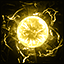
\includegraphics[width=2.5cm]{../Pictures/Gameplay/Spells/Icon/Lumos_spell_icon.png}}         & Illuminates the tip of the caster's wand, allowing the caster to see in the dark. The spell ends if you cast it again or dismiss it as an action. \\ \hline
	\specialcell[p]{\textbf{Reparo}         \\ 
\includegraphics[width=2.5cm]{../Pictures/Gameplay/Spells/Icon/Reparo_spell_icon.png}}         & Seamlessly repairs broken objects. This spell repairs a single break or tear in an object you touch, such as a broken chain link, two halves of a broken key, a torn cloak, or a leaking wineskin. \\ \hline
	\specialcell[p]{\textbf{Accio}         \\ 
\includegraphics[width=2.5cm]{../Pictures/Gameplay/Spells/Icon/Accio_spell_icon.png}}         & Summons a familiar object towards the caster by describing it or naming it. \\ \hline
\end{tabular}

\subparagraph{Level 1} 
Low level spells \\
\begin{tabular}{ p{3cm}p{14cm} } \hline
	\specialcell[p]{\textbf{Wingardium} \\ \textbf{Leviosa}         \\ 
\includegraphics[width=2.5cm]{../Pictures/Gameplay/Spells/Icon/Wingardium_spell_icon.png}}         & Makes objects fly, or levitate. \\ \hline
	\specialcell[p]{\textbf{Fumos}         \\ 
\includegraphics[width=2.5cm]{../Pictures/Gameplay/Spells/Icon/Fumos_spell_icon.png}}         & It's a charm used to create a defensive cloud of smoke from the wand that hinders visibility. \\ \hline
\end{tabular}                                                                                                                                 

\subparagraph{Level 3}                                                                                                                        
Medium spells \\                                                                                                                              
\begin{tabular}{ p{3cm}p{14cm} } \hline  
	\specialcell[p]{\textbf{Alohomora}         \\ 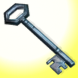
\includegraphics[width=2.5cm]{../Pictures/Gameplay/Spells/Icon/Alohomora_spell_icon.png}}         & Unlocks doors and other locked objects. \\ \hline  
	\specialcell[p]{\textbf{Colloportus}         \\ 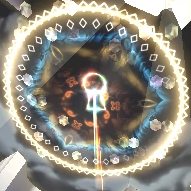
\includegraphics[width=2.5cm]{../Pictures/Gameplay/Spells/Icon/Colloportus_spell_icon.png}}         & Locks doors and all things that can be locked. \\ \hline                                                                                             
\end{tabular}                                                                                                                                 

\subparagraph{Level 5}                                                                                                                        
Greater spells \\                                                                                                                             
\begin{tabular}{ p{3cm}p{14cm} } \hline
	\specialcell[p]{\textbf{Revelio}         \\ 
\includegraphics[width=2.5cm]{../Pictures/Gameplay/Spells/Icon/Revelio_spell_icon.jpg}}         & Reveals secrets and occulted information about a person or object. \\ \hline   
	\specialcell[p]{\textbf{Transfiguration}         \\ 
\includegraphics[width=2.5cm]{../Pictures/Gameplay/Spells/Icon/Transfiguration_spell_icon.png}}         & This spell transforms a creature or an object that you can see within range into a new form. An unwilling creature must make a Wisdom saving throw to avoid the effect. \\ \hline                                                                                                  
\end{tabular}                                                                                                                                 

\subparagraph{Level 7}                                                                                                                        
Superior spells \\                                                                                                                            
\begin{tabular}{ p{3cm}p{14cm} } \hline
	\specialcell[p]{\textbf{Apparate}         \\ 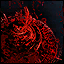
\includegraphics[width=2.5cm]{../Pictures/Gameplay/Spells/Icon/Apparate_spell_icon.png}}         & Magically transports the caster to another location instantaneously. \\ \hline                                                                                                  
\end{tabular}

\subparagraph{Level 8} 
Supreme spells \\
\begin{tabular}{ p{3cm}p{14cm} } \hline
	\specialcell[p]{\textbf{Portkey}         \\ 
\includegraphics[width=2.5cm]{../Pictures/Gameplay/Spells/Icon/Portkey_spell_icon.png}}         & Turns an object into a portkey. \\ \hline
\end{tabular}

\pagebreak
